\chapter{Background}
\label{chap:background}
We will start by discussing the background and related work relevant to this thesis.
For this, we provide an overview of Time Series Forecasting, Prior fitted networks, and finetuning.
\section{Time Series Forecasting}
\label{sec:timeseriesforecasting}
Many processes in industry and also in science can be described by time series data, such as stock prices, weather, etc.
Developing accurate forecasting pipelines based on machine learning is critical to many decision-making processes in various contexts.
Here, we start by giving a formal definition of time series data and our problem setup before we discuss how we treat time series as tabular data.
\subsection{Definition}
\subsubsection{Time Series}
A time series is a sequence of values observed over a period of time represented as $X=\{x_1, x_2, …, x_n\} \in \mathbb{R}^{d \times n}$ where $n$ is the number of temporal observations and $d$ the number of observed values at time point $t$.
One value $x_i$ is a vector of $d$ values observed at time $i$ \citep{wang2024deep}.

Formally, a time series consists of 4 components: A trend $t_t$ which sets the base direction of a time series,
a season component $s_t$ explaining development over a specific period of time,
a cyclic component $z_t$ that describes bigger periodicities and is characterized by fluctuations that tend to be irregular but predictable over the long term,
and a noise component $\epsilon_t$ which adds random fluctuations to the time series \citep{liu2024deep}.
All of these components can be assembled either by adding $x_t = t_t + z_t + s_t + \epsilon_t$ or multiplying $x_t = t_t \cdot z_t \cdot s_t \cdot \epsilon_t$ to create a time series \citep{Dagum2006}.
The multiplicative approach can also be converted to an additive approach by applying the logarithm.
\subsubsection{Time Series Forecast}
In transformer-based time series forecasting, a supervised task consists of a context window $X_{train} \in \mathbb{R}^{d \times n}$ with targets $y_{train} \in \mathbb{R}^{1 \times n}$, where $n$ is the context length, and a forecast window $X_{test} \in \mathbb{R}^{d \times m}$ with targets $y_{test} \in \mathbb{R}^{1 \times m}$, where $m$ is the forecast horizon.
The problem for most time series forecasting algorithms and models is that they require a significant amount of training data to fit the specific time series.
Since available data is limited in many applications, pretrained foundation models are promising \citep{wang2024deep}.
%- hier noch mehr über https://arxiv.org/pdf/2202.07125
%- insights geben welche arten es gibt von forecasting modellen
%- attention vielleicht kurz ansprechen?
%- vielleicht so wie in computational intelligence vorgehen mit windows auch noch
%- generell mal schauen wo noch so time series forcasting erklärt wird
%- while tabpfn was a proof of concept tabpfnv2 was sota
\subsection{Time Series as Tabular Data}
\label{subsec:time_series_as_tabular}
Since time series data is very similar to tabular data, it gives rise to the idea of applying TabPFN to time series tabular data.
A key challenge is that time series data exhibits temporal dependencies, which fundamentally differ from the i.i.d. assumptions commonly made in tabular learning.
Typically, $X_{train}$ and $X_{test}$, both in $\mathbb{R}^{n \times 1}$, consist only of timestamps that progress at a fixed frequency.
Therefore, this information is often not used in time series forecasting, and only $y_{train}$ and $y_{test}$ are used.
But it is impossible to do a forward pass with TabPFN with time series data in the format $D = \{(x_1, y_1),…,(x_n, y_n)\} \in \mathbb{R}^{n \times 2}$, as it would not be able to understand the time-related dependencies of the data because TabPFN was not trained with timestamp data \citep{hollmann2025accurate}. % and is permutation invariant.
To resolve this issue, TabPFN-TS introduces lightweight temporal featurization.
$X_{train}$ and $X_{test}$ are both transformed to hold a greater amount of features than just the timestamp.
\citet{hoo2025tables} uses running index, calendar features, and automatic season features, which are used in this thesis as well and will be further explained in~\ref{subsec:tabpfnts}.
Other types of featurization can also be applied, but need further study \citep{hoo2025tables}.
\subsection{Benchmark}
\subsubsection{GIFT-Eval}
GIFT-Eval(\textbf{G}eneral T\textbf{I}me Series \textbf{F}orecas\textbf{T}ing Model \textbf{Eval}uation) is a time series forecasting benchmark consisting of 23 datasets with over 144,000 time series.
It is one of the first time series forecasting benchmarks that generalizes time series forecasting by providing a mix of datasets from different domains with varying forecast horizons, context lengths, frequencies, windows, and univariate or multivariate data.
Furthermore, the authors provided guidance to split the time series of each dataset into train, validation, and test data, which we will use throughout the whole finetuning process \citep{aksu2024giftevalbenchmarkgeneraltime}.\footnote{\url{https://github.com/SalesforceAIResearch/gift-eval}}
\subsection{Other Data Sources}
\subsubsection{autogluon/chronos-datasets}
We take 4 additional datasets from the autogluon chronos-datasets dataset collection to have a better basis of datasets we will finetune TabPFN-TS with when we are using multiple datasets \citep{ansari2024chronos}.
\section{Prior-data Fitted Networks}
Tabular foundation models or prior fitted networks have become indispensable when it comes to solving downstream tabular data forecasting tasks.
As the enhancement of such models will be examined in this thesis, we will have to look at prior work regarding these models.
\subsection{Definition}
In recent years, transformers have shown great results on tasks where large amounts of data are available.
But not in every task is there enough data to train such a model.
\newline
For such a case, \citet{muller2021transformers} introduces prior fitted networks, a transformer-based architecture that trains on artificial tasks generated from a prior.
This generated data is set to imitate the real-world tasks the model is supposed to solve later, so that the model learns to learn on datasets generated by the prior.
Using this generative process to produce large amounts of training data, \citet{muller2021transformers} show that this type of architecture effectively approximates the posterior predictive distribution (PPD).
\newline
The authors define a prior $p(t)$ over tasks, which is used to generate artificial training tasks, where $t$ denotes the task from which the model samples data.
These training tasks consist of an arbitrary supervised dataset $D=\{x_i, y_i\}^n_{i=1}$ of size $n$.
\newline
Using the components mentioned above and the posterior $p(t, D)$ defined by the authors via Bayes’ theorem, the posterior distribution is defined as follows
\[
p(y | x, D) = \int_{t} p(y|x, t)p(t, D)
\]
where $y$ is the output for a new input $x$ \citep{muller2021transformers}.
\newline
Traditionally, the approximation of this distribution is done by approximating the posterior $p(t, D)$ and then deriving the approximation of the PPD from it.
A PFN approximates the PPD directly from dataset samples as follows.
\newline
A PFN accepts data in the following format.
A dataset $D = {(x_i, y_i)}^n_{i=1}$ and a query $x$, for which the labels $y$ will be predicted in the task.
For pretraining, datasets are sampled by $D \sim p(D)=\int_t p(D, t)p(t)dt$, and the query $x$ and test label $y$ are extracted from it.
The model $q_{\theta}$ predicts the target $y$. The negative log-likelihood
\[
\ell_{\theta} = \mathbb{E}_{D \cup \{x, y\} \sim p(D)} \left[ -\log q_{\theta}(y \mid x, D) \right]
\]
is used as the loss function, where $D \cup \{x, y\}$ denotes a dataset of size $|D|+1$ sampled from $p(D)$. The loss is minimized using stochastic gradient descent.
\citet{muller2021transformers} showed that minimizing the Prior-Data NLL yields an approximation of the PPD in terms of cross-entropy and KL-Divergence.

In this architecture, priors are indispensable.
They provide the basis of a PFN and represent an assumption of how the data is represented in the real world, where $\phi$ is a hypothesis, which is sampled with $\phi \sim p(\phi)$ and normally represents either the whole algorithm that generates the data or the hyperparameters that are used to generate the data \citep{hollmann2022tabpfn}.
We will now investigate how to build such priors.
\subsection{Prior Building}
\label{subsec:prior_building}
\subsubsection{TabPFN Prior}
The prior of TabPFN is implemented by using a Structural Causal Model (SCM).
\newline
An SCM is a collection of $k$ structural assignments $Z:=(z_1, …, z_k)$ which are represented by nodes in a directed acyclic graph where $z_i = f_i(z_{PA\mathcal{G}(i)}, \epsilon)$.
$f_i$ is a (nonlinear) deterministic function, $PA\mathcal{G}(i)$ represents the parent nodes of node $i$ in graph $\mathcal{G}$, and $\epsilon_i$ is a noise variable. \newline
To generate a new artificial dataset, there has to be a subset of nodes selected, from which the features and targets will later be extracted.
Then, random noise is propagated through the graph, where the noise is sampled either from a normal distribution or from a uniform distribution with varying degrees of non-independence for each sample.
At each edge of the graph, the corresponding function $f_i$ will be applied, and Gaussian noise will be added to the data.
These functions can be activation functions like ReLU or sigmoid, but can also be discretization methods to generate classification features.\newline
After traversing the graph, the targets and features for one sample will be extracted at the corresponding node.
This process will be repeated for every sample of a dataset.
Throughout the process, the extraction nodes and the function will stay the same \citep{hollmann2025accurate}.

\subsubsection{ForecastPFN Prior}
The works of \citet{dooley2023forecastpfn} are especially relevant for this thesis since they developed a prior that generates artificial time series data.
It creates time series data from three components: periodic trends, global trends, and noise.
\newline
Firstly, the global trend is being created via a linear and exponential component controlled by the coefficients $m_{lin}$, $c_{lin}$, $m_{exp}$, and $c_{exp}$.
\[
\text{trend}(t)=(1+m_{lin} \cdot t + c_{lin})*(m_{exp} \cdot c_{exp}^t)
\]
All the components named above are sampled the following: $m_{lin}, m_{exp} \sim \mathcal{N}(\mu_m, \sigma_m)$; $c_{lin} \sim \mathcal{N}(0, \sigma_{lin})$; $c_{exp} \sim \mathcal{N}(0, \sigma_{exp})$
\newline
    Next, the seasonal component is created by the product of a weekly, a monthly, and a yearly seasonal component:
\[
\text{seasonal}(t) = \text{seasonal}_{week}(t) \cdot \text{seasonal}_{month}(t) \cdot \text{seasonal}_{year}(t)
\]
Where
\[
\text{seasonal}_{\nu}(t)=1+m_{\nu} \sum^{\lfloor p_{\nu}/2 \rfloor}{f=1} \left[c{f, \nu} sin\left(2\pi f \frac{t}{p_\nu}\right) + d_{f, \nu}cos\left(2 \pi f \frac{t}{p_{\nu}}\right)\right]
\]
corresponds to the respective seasonal period $\nu \in {\text{week, month, year}}$. $p_{week} = 7$, $p_{month}=30.5$, $p_{year}=365.25$ and $c_{f, \nu}, d_{f, \nu} \sim \mathcal{N}(0, 1/f)$ which are both dependent on $f$ and $\nu$.
\newline
After sampling both the seasonal and global trend components, only the noise component $z_t$ has to be sampled.
\[
z_t = 1 + m_{noise}(z - \overline{z})
\]
where $z \sim \text{Weibull}(1, k)$ and $\overline{z} = (ln(2))^{1/k}$.
\newline
After sampling all the base components, the timestamp $y_t$ is composed of the product of all the components mentioned above.
\[
y_t = \text{trend}(t) \cdot \text{seasonal}(t) \cdot z_t
\]

The noise component is multiplied, not added, to make the scale of it independent of the scale of the other components.
In addition, the Weibull distribution creates the chance to parameterize between the Gaussian and the exponential distribution, both of which are common in real-world time series \citep{dooley2023forecastpfn}.
\newline
There are three different observation periods (i.e., the frequency at which data is recorded): daily, monthly, and yearly.
These periods are independent of the time series generation process and primarily serve to provide the mod  el with additional context across different periodicities.

\subsection{TabPFN}
Researchers from the Universities of Freiburg and Charité Berlin developed TabPFN \citep{hollmann2022tabpfn}: A prior fitted network which builds up on a 12-layer transformer and is able to solve tabular classification or regression tasks in a single forward pass.

Contrary to conventional supervised deep learning approaches, in which models are trained from scratch for every dataset, TabPFN is pretrained on a large amount of artificially generated training tasks only once.
Normally in machine learning, a training task consist of a tuple with the following scheme $(x_{train}, y_{train})$ in which $x_{train}  \in \mathbb{R}^{1 \times d}$ represents the input data with $d$ features and $y_{train} \mathbb{R}^{1}$ the corresponding labels.
However, this is slightly different for TabPFN, as tabular data consists of multiple tasks/samples.
So one datapoint, which is used to train TabPFN, is a set of training samples $D_{train} = \{(x_1, y_1), …, (x_n, y_n)\}$.
\newline
The key problem with this type of training is that tabular datasets of this size are extremely rare and often not accessible without breaking privacy laws.
To obtain a sufficient amount of data to train TabPFN with, a prior is used.

The pre-training tasks are generated by a prior, which is a generative process that allows us to efficiently sample artificial tabular datasets of different shapes and with different characteristics.
To be more precise, TabPFN uses Structural Causal Models, which are based on graphs to generate this data (see \autoref{subsec:prior_building}).
To obtain the best result, the prior has to cover a heterogeneous set of datasets to be able to generalize to real-world datasets.
This can be achieved by sampling different characteristics of the underlying graph from the prior’s distribution.

TabPFNs architecture is a combination of the original transformer encoder and the PFN architecture.
The most important part in the architecture is that it uses inter-feature and sample attention.
This enables the model to be invariant in the order of samples and features.
But unlike fully connected attention, test samples are not allowed to attend to each other but only to the training data, so that test samples do not influence each other \citep{hollmann2025accurate}.

TabPFN training and inference differ fundamentally from traditional deep learning algorithms.
As previously mentioned, for TabPFN, one training sample consists of a set of samples $\{x_i, y_i\}^n_{i=1}$.
Instead of doing one forward pass for each input data point at inference time, the pretrained TabPFN model receives $D_{train} = \{(x_1, y_1), …, (x_n, y_n)\}$ as context and predicts $y_{test}$ based on $X_{test}$ in one single forward pass.
So fitting and prediction is performed in one forward pass.

Instead of returning a single point estimate in regression, TabPFN outputs a target distribution that captures the uncertainty of the predictions.
The boundaries of this predictive distribution are determined by selecting the 1/5000 quantiles of the prior distribution on which TabPFN was pretrained, as shown in figure~\ref{fig:bardist_hospital}.
These boundaries are normalized, as TabPFN was trained on z-normalized data during pretraining, but are later reverted by applying the inverse transformation to the bucket boundaries.
During training for regression, the entire distribution is used to minimize the mean negative log density, whereas during inference, the median of the predictive distribution is typically used.
\begin{figure}[h]
\centering
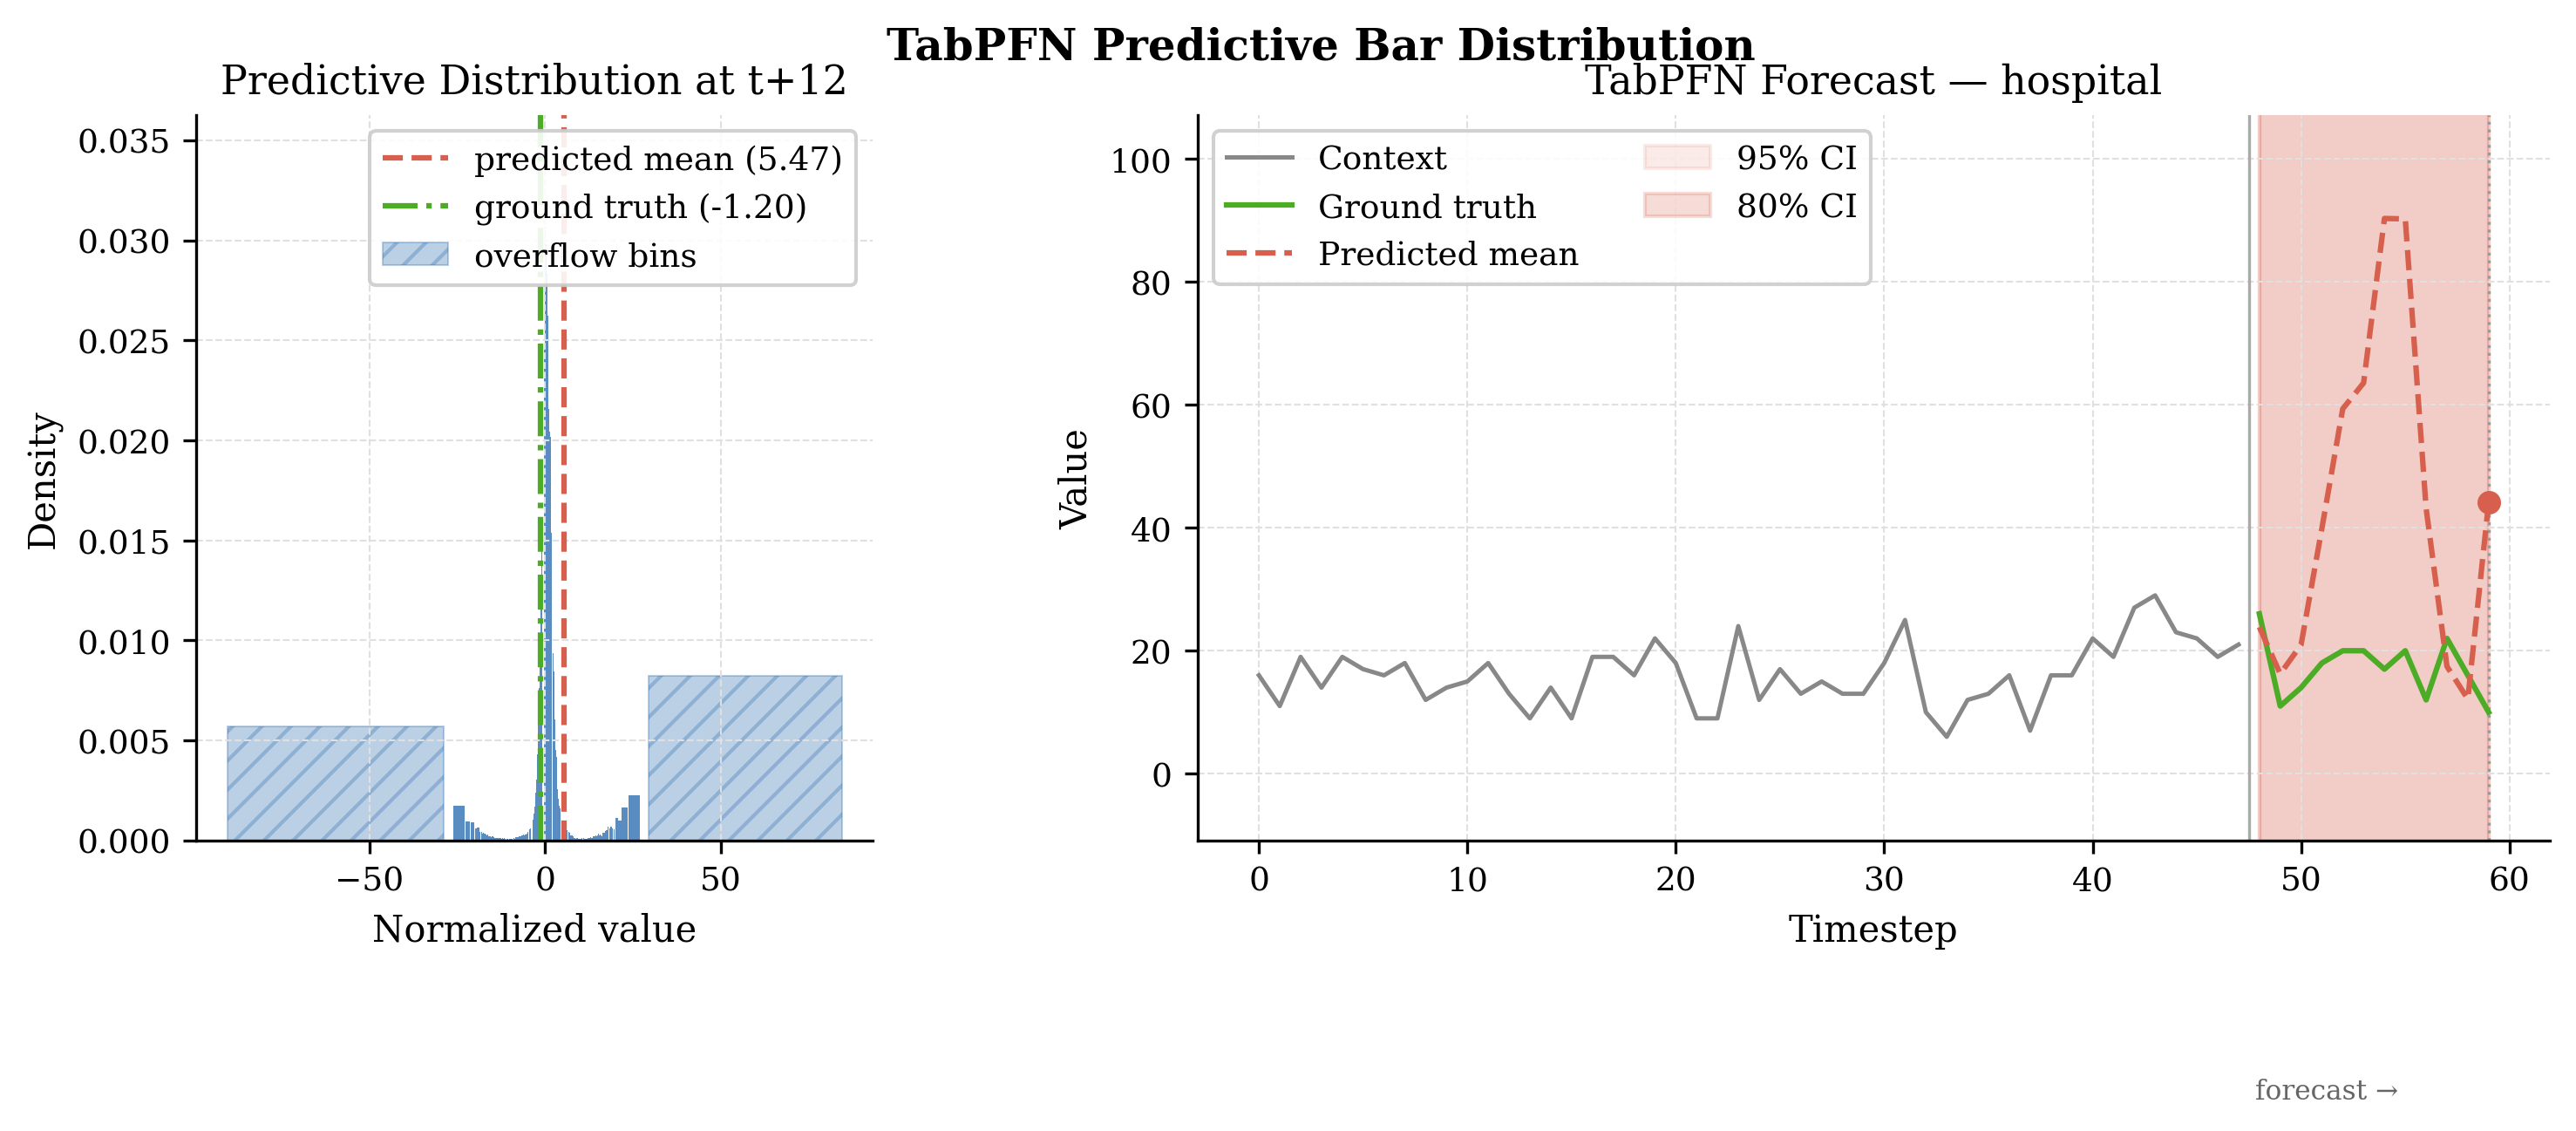
\includegraphics[width=0.8\textwidth]{pictures/bardist_hospital.png}
\caption{TabPFN Predictive Bar Distribution on the hospital dataset for the last predicted value. The boxes left and right in the bar distribution are cumulative densities for the given threshold.}
\label{fig:bardist_hospital}
\end{figure}
%classification point estimation?
\newline

TabPFN especially outperforms comparable models like CatBoost, Autogluon, etc.\ on small to medium-sized datasets with up to 10000 samples and 500 features \citep{hollmann2025accurate}.
This limitation results from the fact that the prior used during pretraining generated datasets only up to this size.\newline
Compared to gradient-boosted decision trees, a 3000x faster performance in regression and a 5140x faster performance in classification on a NVIDIA RTX 2080 Ti has been observed \ citep {hollmann2025accurate}. \newline
Another interesting detail researchers have discovered is that TabPFN works out of the box without any necessary hyperparameter tuning, especially in classification.
But even when using hyperparameter search, TabPFN showed remarkable and efficient results: After just 300s of hyperparameter tuning, TabPFN outperforms Autogluon, which was also hyperparameter-tuned, but for 4 hours.

While TabPFN achieves strong performance on tabular benchmarks, its generalization to other data modalities is not guaranteed.
In particular, its performance on time series data depends on how effectively temporal information is encoded into tabular features.
\subsection{TabPFN-TS}
\label{subsec:tabpfnts}
\citet{hoo2025tables} introduce TabPFN-TS: A model that combines TabPFN with lightweight feature engineering to enable both point and probabilistic forecasting.
Point forecasting predicts a single value, while probabilistic forecasting returns a distribution of quantiles.
As mentioned in \autoref{subsec:time_series_as_tabular}, \citet{hoo2025tables} split these data into the following features.
\subsubsection{Running Index}
The Running index is one feature that serves as an index for each observation in the time series to provide an effective way to track progression in time series.
The first Observation has a running index of 0, the next has a running index of 1, and so on.
Formally, this adds the following feature to $X$:
\[
\Phi_{index}(t) = t \in \mathbb{R}
\]
\subsubsection{Calendar Features}
To give TabPFN a better understanding of the temporal cycle that is used in our society, the timestamp data is encoded into eight cyclic calendar components.
These are: second of minute, minute of hour, hour of day, day of week, day of month, day of year, week of year, and month of year.
To encode these values into cyclic values, the sine and cosine functions are both separately applied to each calendar component.
Additionally, the current calendar year is also included as a non-cyclic component.
So each timestamp t is encoded in the following:
\[
\Phi_{cal}(t)=\left(cos\left(\frac{2 \pi t}{P_1}\right), sin\left(\frac{2 \pi t}{P_1}\right), …, cos\left(\frac{2 \pi t}{P_8}\right), sin\left(\frac{2 \pi t}{P_8}\right), year(t)\right) \in \mathbb{R}^{17}
\]
With ${P_{i}}^8_{i=1}$ being the periods of the calendar components.
\subsubsection{Automatic Season Features}
Most time series exhibit domain-specific cycles that cannot be captured by calendar features.
To also take these cycles into account, \citet{hoo2025tables} introduces an algorithm that extracts the top-k periodicities and encodes them as features.
At first, the series is detrended with the use of a simple least squares regression.
After that, to reduce spectral leakage and improve frequency resolution, a Hann window is applied, and the windowed signal is zero-padded by a factor of two.
Now, to extract the features, the real-valued Fourier transformation is calculated and the zero-frequency component, which corresponds to the mean value, is removed \citet{hoo2025tables}.
After that, the k largest spectral peaks by magnitude $f_1, …, f_k$ are selected, and the features are calculated as follows:
\[
\Phi_{auto}(t) = (cos(2\pi f_1 t), sin(2 \pi f_1 t), …, cos(2\pi f_k t), sin(2 \pi f_k t)) \in \mathbb{R}^{2k}
\]
\subsubsection{Time-varying Covariates (when available)}
Also, known time-varying covariates like holidays can be taken into account and are denoted as follows:
\[
z_{1:C+H} = [z_1, …, z_{C+H}]
\]
where $z_t \in \mathbb{R}^{D_{z}}$ represents $D_z$ external variables observed at time \textbf{t}
\newline
\
Each timestamp $x_t \in X=X_{train} \cup X_{test}$ is now defined as:
\[
x_t = \Phi_{index}(t) \oplus \Phi_{cal}(t) \oplus \Phi_{auto}(t) \oplus z_t \in \mathbb{R}^{18+2k+D_z}
\]

To avoid much slower inference, TabPFN-TS does not rely on lagged or auto-regressive features like moving averages or lag terms as comparable models do.
\newline
With the help of this encoding, TabPFNv2 is able to achieve state-of-the-art performance in covariate-informed forecasting and competitive accuracy in univariate time series forecasting.
To evaluate TabPFN-TS, the GIFT-EVAL benchmark has been used \citep{hoo2025tables}.
\newline
In this thesis, we will use the code of the featurization as well as the evaluation to implement our finetuning pipeline.\footnote{\url{https://github.com/PriorLabs/tabpfn-time-series}}
\subsection{Finetuning}
\subsubsection{Definition}
Fine-tuning is commonly used in deep learning to adapt pretrained foundation models to specific tasks.
\newline
Foundation models are typically pretrained on large and heterogeneous datasets to achieve strong performance across a wide range of tasks within a given domain.
To further improve performance on a specific real-world dataset, the model is finetuned by training on that dataset.
\newline
Specifically for TabPFN, which was trained on artificial data created from a prior, it is crucial for finetuning to use a real-world dataset \citep{rubachev2025finetuning}.

Finetuning can improve performance on specific datasets, but may also lead to overfitting or reduced generalization.
In particular, improvements are often dataset-specific and may not transfer to other tasks.
Training on multiple datasets introduces extra variability, which may benefit generalization but complicates optimization.
\subsubsection{Related Work}
\citet{rubachev2025finetuning} lists two main ways of finetuning methods popular with tabular foundation models.
The first one is full finetuning, in which all parameters are updated as in the pretraining process.
The other one is parameter-efficient finetuning (PEFT), which is often used for LLM adaptation, since they have a significantly larger amount of parameters (TabPFN ~7M vs GPT-3 ~175B)\citep{brown2020language, hollmann2025accurate}.
The authors also found that full finetuning, due to its similar approach for improved retrieval-based assessments, is the superior way of finetuning TabPFNv2.
For this reason, we will also only investigate full finetuning in this thesis.\newline
While finetuning on one dataset improves performance on this specific dataset, finetuning on many datasets at once, like \citet{Hollmann_2025} did, showed significant performance boosts in downstream tasks.
They used the original TabPFNv2 configuration that was pretrained on artificial data and used a diverse amount of datasets for improvements.
Furthermore, they called this method `continued pretraining’, which is contrary to our assumption for this thesis that finetuning solely relies on training on real-world datasets, while continued pretraining uses artificial datasets from a prior.

\subsection{Continued Pretraining}
\subsubsection{Definition}
As mentioned above, we define continued pretraining as further training a foundation model on a domain-specific prior with the goal of improving its performance.
\subsubsection{Related Work}
There has been limited work on continued pretraining with domain-specific priors. However, \citet{kolberg2025tabpfn} showed that continuing to pretrain TabPFNv2 on a similar modality (tabular data with high feature dimensionality and low sample count) leads to decreased performance on datasets that do not exhibit these characteristics.
This demonstrates that while continued pretraining can be beneficial, its effects are highly dependent on the alignment between the prior and the target data distribution, indicating that possible benefits have not yet been fully explored.
\newline

